
\documentclass[12pt,a4paper,usenames,x11names,compress]{beamer}
\usetheme[numbering=none,block=fill,progressbar=foot]{metropolis}
\useoutertheme{metropolis}
\setbeamercolor{frametitle}{bg=DarkOrange1}
\setbeamercolor{progress bar}{fg=Chocolate1,bg=SkyBlue1}
\setbeamercolor{block title}{fg=white,bg=RoyalBlue4}
\setbeamercolor{block body}{fg=black,bg=SteelBlue4!20}
\setbeamercolor{normal text}{fg=black}
\usepackage{array}
\newcolumntype{P}[1]{>{\centering\arraybackslash}p{#1}}
\usepackage{amsmath}
\usepackage{amssymb}
\usepackage{commath}
%\usepackage{xcolor}
\usepackage{color}
\usepackage[utf8]{inputenc}
\usepackage[english, spanish]{babel}
\usepackage[T1]{fontenc}
\usepackage{lmodern}
\usepackage{ragged2e}
\usepackage{hyperref}
\usepackage{siunitx}
\usepackage{colortbl}
\usepackage{metalogo}
\usepackage{multirow}
\usepackage{tikz}
\usetikzlibrary{shapes.geometric, arrows}
\usetikzlibrary{positioning}
\usetikzlibrary{decorations.pathmorphing,calc,shadows.blur,shadings,mindmap}
\usepackage{smartdiagram}


\tikzset{
  my blur shadow layer/.style={
    preaction={fill=black,fill opacity=.025,transform canvas={xshift=#1,yshift=-1*#1}},
  },
  my blur shadow/.style={
    my blur shadow layer/.list={.3pt,.6pt,...,2.7pt},
  },
}

\tikzstyle{drawrect}=[draw, rectangle,anchor=west, minimum height=2,
  minimum width=8,fill=gray!20,text width=4cm]



\tolerance=1
\emergencystretch=\maxdimen
\hyphenpenalty=10000
\hbadness=10000
\setbeamersize{text margin left=10pt,text margin right=20pt}


\author[A. Vallone]{{\Large Andr\'{e}s Vallone} \inst{1}}
\institute{\inst{1}{\normalsize Escuela de Ciencias Empresariales}}
\title{\textcolor{DarkOrange1}{Manejo de repositorios en Github}}
\subtitle{\textcolor{white}{Taller de desarrollo de habilidades de investigaci\'{o}n\hfill 2023}}
\titlegraphic{%
  
\includegraphics[scale=.3]{eciem_1.png} \hfill 
\includegraphics[scale=.05]{github.png}
}
\date{2023}
\makeatletter
\setbeamertemplate{title page}{
  \begin{minipage}[b][\paperheight]{\textwidth}
    \vfill%
    \ifx\inserttitle\@empty\else\usebeamertemplate*{title}\fi
    \ifx\insertsubtitle\@empty\else\usebeamertemplate*{subtitle}\fi
    \usebeamertemplate*{title separator}
    \ifx\beamer@shortauthor\@empty\else\usebeamertemplate*{author}\fi
    \ifx\insertinstitute\@empty\else\usebeamertemplate*{institute}\fi
    \vfill
    \ifx\inserttitlegraphic\@empty\else\inserttitlegraphic\fi
    \vspace*{1cm}
  \end{minipage}
}



\makeatletter
\setlength{\metropolis@titleseparator@linewidth}{2pt}
\setlength{\metropolis@progressonsectionpage@linewidth}{2pt}
\setlength{\metropolis@progressinheadfoot@linewidth}{2pt}
\makeatother


\makeatletter
\defbeamertemplate*{section page}{mytheme}[1][]{
  \centering
  \begin{minipage}{22em}
    \raggedright
    \usebeamercolor[fg]{section title}
    \usebeamerfont{section title}
    \insertsectionhead\\[-1ex]
    \usebeamertemplate*{progress bar in section page}
    \par
    \ifx\insertsubsectionhead\@empty\else%
      \usebeamercolor[fg]{subsection title}%
      \usebeamerfont{subsection title}%
      \insertsubsectionhead
    \fi
    \vskip0.5cm
        \begin{center}
        
\includegraphics[width=.5\textwidth]{eciem_1.png}%
        \end{center}
  \end{minipage}
  \par
  \vspace{\baselineskip}
}
\makeatother








\setbeamercolor{background canvas}{bg=white}
\begin{document}
{
\beamertemplateshadingbackground{white}{Blue4}
\begin{frame}
%\centering
%\includegraphics[scale=.3]{logo_eco.png}
\titlepage
\end{frame}
}

\part{Repaso}

\section{Repaso}
\begin{frame}{Repaso\hfill 
\includegraphics[scale=.1]{eciem.png}}
\begin{itemize}
\item Conocimos que era Git y control de Cambios
\item Conocimos que era GitHub y Github Desktop
\item Hicimos nuestra cuenta en GitHub 
\item Instalamos y configuramos Git y GitHub Desktop
\item Creamos un repositorio usando la aplicación web de GitHub
\item Modificamos el README.md en nuestro repositorio generando un commit
\end{itemize}
\end{frame}

\begin{frame}{Recordando conceptos \hfill 
\includegraphics[scale=.1]{eciem.png}}
\begin{columns}
\column{0.3\textwidth}
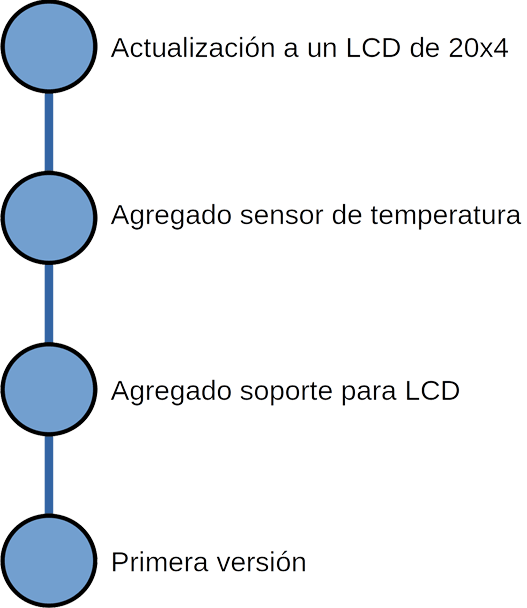
\includegraphics[scale=.23]{commit.png} 
\column{0.7\textwidth}
\begin{itemize}
\justifying
 \item Git almacena cada vez que se realiza y confirma (commit) algún cambio
 \item Cada uno de los nodos representa un cambio confirmado (commit).
 \item A una sucesión de commits se le conoce como rama (branch)
 \item La rama principal del proyecto es la rama master
 \item La master es la rama estable, por tanto se trata de no modificarla.
 \item Para hacer cambios sin modificar la master, es posible crear una nueva rama.
\end{itemize}
\end{columns}
\end{frame}


\begin{frame}{Recordando conceptos\hfill 
\includegraphics[scale=.1]{eciem.png}}
\begin{columns}
\column{0.4\textwidth}
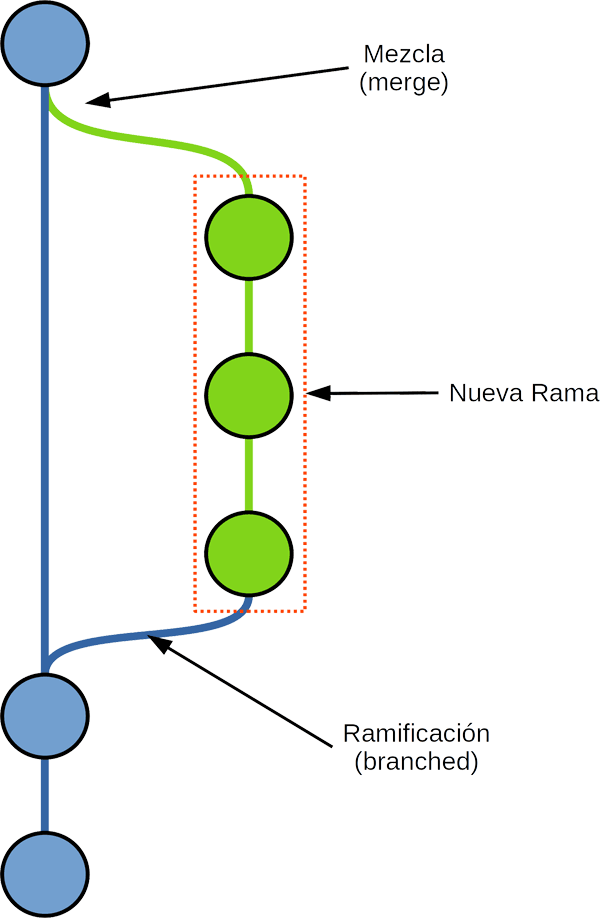
\includegraphics[scale=.22]{commit_rama.png} 
\column{0.6\textwidth}
\begin{itemize}
\justifying
 \item Cada uno de colaboradores puede tener una rama propia y modificar el proyecto.
 \item Cada una de las ramas tendrá su propia historia.
 \item Los cambios en las ramas son independientes de la master.
 %\item La master es la rama estable, por tanto el master es siempre estable.
 \item Para incorporar los cambios al master se debe solicitar un merge
\end{itemize}
\end{columns}
\end{frame}

\section{Usando el repositorio}

\begin{frame}{Resultados esperados de la sesión\hfill 
\includegraphics[scale=.1]{eciem.png}}
\begin{itemize}
\item Se espera que al final de la sesión usted sea capaz de:
\begin{itemize}
\justifying
\item sincronizar el repositorio localmente
\item subir y bajar información de un repositorio
\item clonar un repositorio 
\item Hacer una rama y un merge al master
\end{itemize} 
\end{itemize}
\end{frame}
%
%\section{Git y GitHub}
%\begin{frame}{¿Qué es Git? \hfill 
\includegraphics[scale=.1]{eciem.png}}
%\begin{columns}
%\column{.8\textwidth}
% \begin{itemize}
% \justifying
%    \item Git es un software de control de versiones distribuido,  optimiza el trabajo en proyectos.
% \end{itemize}
%
%\column{.2\textwidth}
%
\includegraphics[scale=.1]{git.png}  
%\end{columns}
%\begin{itemize}
%\justifying
%\item Un software de control de versiones: registra cambios realizados en un archivo o conjunto de archivos en tiempo, entonces se puede recuperar versiones específicas.
%\item Los proyectos se almacenan en repositorios que contiene los archivos del proyecto junto a todo el historial de cambios. 
%\item Es distribuido, por lo que cada desarrollador tiene una clon local del repositorio principal 
%\end{itemize}
%\end{frame}
%
%
%\begin{frame}{¿Qué es Git?\hfill 
\includegraphics[scale=.1]{eciem.png}}
%\begin{columns}
%\column{0.3\textwidth}
%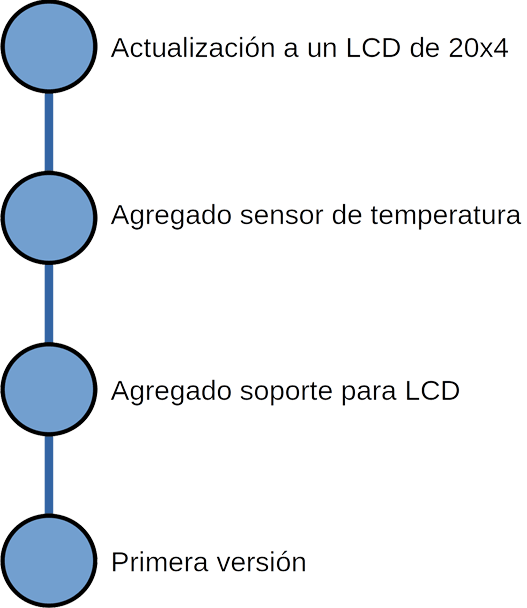
\includegraphics[scale=.23]{commit.png} 
%\column{0.7\textwidth}
%\begin{itemize}
%\justifying
% \item Git almacena cada vez que se realiza y confirma (commit) algún cambio
% \item Cada uno de los nodos representa un cambio confirmado (commit).
% \item A una sucesión de commits se le conoce como rama (branch)
% \item La rama principal del proyecto es la rama master
% \item La master es la rama estable, por tanto se trata de no modificarla.
% \item Para hacer cambios sin modificar la master, es posible crear una nueva rama.
%\end{itemize}
%\end{columns}
%\end{frame}
%
%
%\begin{frame}{¿Qué es Git?\hfill 
\includegraphics[scale=.1]{eciem.png}}
%\begin{columns}
%\column{0.4\textwidth}
%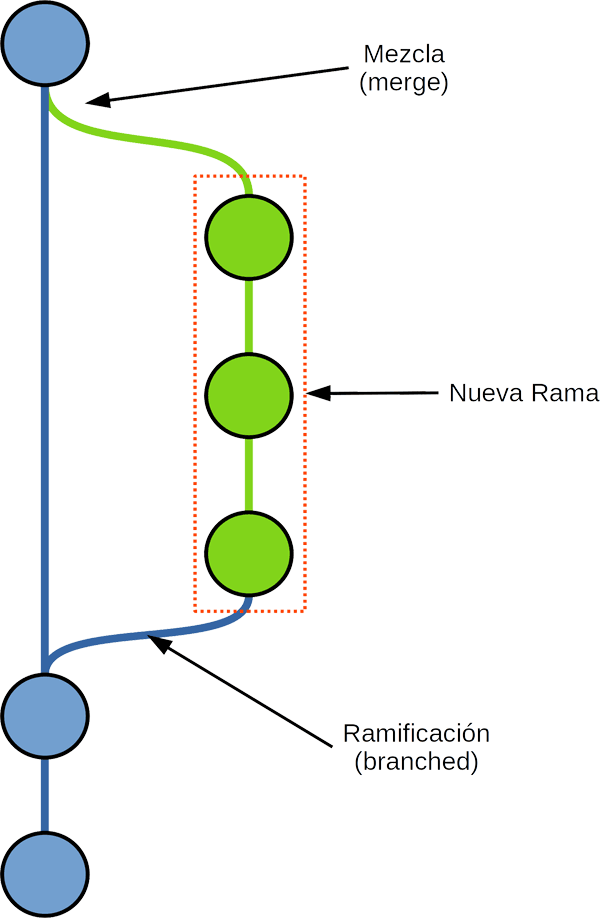
\includegraphics[scale=.22]{commit_rama.png} 
%\column{0.6\textwidth}
%\begin{itemize}
%\justifying
% \item Cada uno de colaboradores puede tener una rama propia y modificar el proyecto.
% \item Cada una de las ramas tendrá su propia historia.
% \item Los cambios en las ramas son independientes de la master.
% %\item La master es la rama estable, por tanto el master es siempre estable.
% \item Para incorporar los cambios al master se debe solicitar un merge
%\end{itemize}
%\end{columns}
%\end{frame}
%
%\begin{frame}{¿Qué es GitHub?\hfill 
\includegraphics[scale=.1]{eciem.png}}
%\begin{columns}
%\column{.8\textwidth}
% \begin{itemize}
% \justifying
%\item Es una plataforma de desarrollo colaborativo para alojar y gestionar proyectos utilizando el sistema de control de versiones Git.
% \end{itemize}
%
%\column{.2\textwidth}
%
\includegraphics[scale=.027]{github.png}  
%\end{columns}
%\begin{itemize}
%\justifying
%\item Se utiliza principalmente para la creación de código fuente (código simple o un programa completo)
%\item GitHub ofrece rasgos similares a los de una red social: Se puede seguir un desarrollador, un proyecto, un tipo de programación 
%\item La plataforma permite que  cualquier persona  sea capaz visualizar el código y colaborar con su desarrollo, es decir, máxima expresión del ``open source''
%\end{itemize}
%\end{frame}
%
%\begin{frame}{¿Para qué me sirve GitHub?\hfill 
\includegraphics[scale=.1]{eciem.png}}
%\begin{itemize}
%\item Es eficiente para
%\begin{itemize}
%\justifying
%\item Alojar base de datos de papers y los códigos de ejecución
%\item Utilizar un sistema de control de cambio en archivos de binarios (\LaTeX, html, Markdown,R, phyton,...) 
%\item Trabajar en simultaneo con otros investigadores en distintas partes de un código
%\item Desarrollar software colaborativamente (Paquetes en R, librerías de phyton,dahboard,...)
%\end{itemize}
%\item Se puede, pero no es lo ideal
%\begin{itemize}
%\justifying
%\item Alojar archivos para difusión.
%\item Usar como control de versión de archivos no binarios.
%\item Usar como backup de archivos.
%\end{itemize}
%\end{itemize}
%\end{frame}
%
%\begin{frame}{¿Qué es GitHub Desktop? \hfill 
\includegraphics[scale=.1]{eciem.png}}
%\begin{center}
%
\includegraphics[scale=.21]{desktop.png} 
%\end{center}%
%\begin{itemize}
%\justifying
%\item Git se utiliza mediante linea de comandos en el terminal o consola
%\item GitHub es Git, por tanto, las lineas de comanda funcionan,  pero se puede utilizar mediante un web browser
%\item GitHub Desktop es una aplicación que te habilita para interactuar con GitHub utilizando una GUI en vez de la línea de comandos o un web browser. 
%\item Es un facilitador de uso de repositorios, es decir tenemos las bondades del Git sin usar comandos.
%\end{itemize}
%\end{frame}
%
%\section{Usando GitHub}
%\begin{frame}{Requisitos \hfill 
\includegraphics[scale=.1]{eciem.png}}
%\begin{enumerate}
%\item Cree su cuenta en GitHub accediendo \href{https://github.com/login}{aquí}
%\item Descargue e instale Git desde \href{https://git-scm.com/downloads}{aquí}
%\item Descargue e instale GitHub Desktop desde \href{https://desktop.github.com/}{aquí}
%\end{enumerate}
%\end{frame}
%

\begin{frame}{Acciones básicas \hfill 
\includegraphics[scale=.1]{eciem.png}}
Existen un conjunto de acciones básicas que se deben conocer al trabajar con repositorios:
\begin{itemize}
\justifying
\item \textbf{pull}: Obtiene los archivos del repositorio remoto y los combina con el local.
\item \textbf{commit}:Crea una entrada en el indice de historiales, establece la versión.
\item \textbf{push}:Envía todos los objetos modificados localmente al repositorio remoto
\item \textbf{clone}: Crea una copia de repositorio GIT de una fuente externa
\item \textbf{fork}:Crea una bifurcación o rama nueva.
\item \textbf{merge}:Fusiona una o más ramas con otra rama activa y crea automáticamente un nuevo commit si no hay conflictos
\end{itemize}
\end{frame}


\end{document}